\documentclass[hyperref={pdfpagelabels=false}]{beamer}
\usepackage{lmodern}
\usetheme{CambridgeUS}

\usepackage[english,brazilian]{babel}
\usepackage{multicol}
\usepackage{textcomp}
\usepackage[alf]{abntex2cite}
\usepackage[utf8]{inputenc}
\usepackage[T1]{fontenc}

\title{Funções}  
\author[Matheus Pimenta]{Matheus Pimenta} 
\institute[UTFPR-CP]{\normalsize Universidade Tecnológica Federal do Paraná \\
	Câmpus Cornélio Procópio
} 
\date{Março de 2019} 
\begin{document}
	
\begin{frame}
\titlepage
\end{frame} 


%\begin{frame}
%\frametitle{Table of contents}
%\tableofcontents
%\end{frame} 


\section{Funções} 


\begin{frame}
\frametitle{Exemplo 01} 

Determine $\frac{f(x+h)-f(x)}{h}$ onde $h \neq 0$, se:
\begin{enumerate}
	\item [a)] $f(x) = 4x^2-5x+7$
	\pause
	\item [b)] $f(x) = \sqrt{x}$
\end{enumerate}

\pause 

\begin{figure}[!htb]
	\centering
	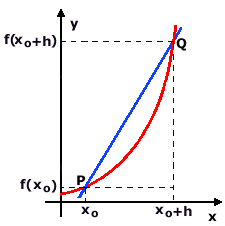
\includegraphics[scale=0.5]{inc.png}
	\caption{Inclinação da reta}
\end{figure}

\end{frame}

\section{Regressão}

\begin{frame}
\frametitle{Exemplo 01}
A tabela a seguir mostra a receita de uma empresa nos primeiros cinco anos de operação.

\begin{table}
	\centering
	\begin{tabular}{|c|c|}
		\hline
		X (anos)	&	Receita (milhares de reais) \\
		\hline
		1			&	$3,50$	\\
		\hline
		2			&	$5,25$	\\
		\hline
		3			&	$9,25$	\\
		\hline
		4			&	$9,75$	\\
		\hline
		5			&	$14$	\\
		\hline		
	\end{tabular}
\end{table}

Determine a equação da reta de regressão para este conjunto de dados e use-a para prever qual será a receita no sexto ano de operação, supondo que a relação entre o tempo de operação e a receita é aproximadamente linear.

\end{frame}

\begin{frame}
\frametitle{Exemplo 02}

Use a planilha do Excel para plotar o gráfico e determinar a fórmula de regressão quadrática que melhor se ajusta à seguinte tabela de dados para a curva de demanda de um certo produto de informática.

\begin{table}
	\centering
	\begin{tabular}{|c|c|}
		\hline
		p	&	q	\\
		\hline
		3	&	66	\\
		\hline
		6	&	58	\\
		\hline
		9	&	50	\\
		\hline
		12	&	43	\\
		\hline
		15	&	37	\\
		\hline
		18	&	31	\\
		\hline
		21	&	25	\\
		\hline
		24	&	20	\\
		\hline
		27	&	16	\\
		\hline
		30	&	12	\\
		\hline
	\end{tabular}
\end{table}

\end{frame}


\begin{frame}
\frametitle{Exemplo 03}

Use a planilha do Excel para plotar o gráfico e determinar a fórmula de regressão quadrática que melhor se ajusta à seguinte tabela de dados para a curva de oferta de um certo produto de informática.

\begin{table}
	\centering
	\begin{tabular}{|c|c|}
		\hline
		p	&	q	\\
		\hline
		3	&	6	\\
		\hline
		6	&	10	\\
		\hline
		9	&	14	\\
		\hline
		12	&	19	\\
		\hline
		15	&	25	\\
		\hline
		18	&	30	\\
		\hline
		21	&	37	\\
		\hline
		24	&	44	\\
		\hline
		27	&	52	\\
		\hline
		30	&	60	\\
		\hline
	\end{tabular}
\end{table}

\end{frame}

\begin{frame}
\frametitle{Exemplo 04}

Determine o preço e a demanda de equilíbrio dos exemplos $02$ e $03$, tente mostrar isso graficamente também.

\end{frame}

\begin{frame}
\frametitle{Exemplo 05}

Alguns dados, quando são plotados em gráficos de pontos, parecem de ajustar melhor a um polinômio cúbico ou de grau mais elevado. Utilizando uma planilha do Excel, encontre o melhor ajuste para os dados da tabela:

\begin{table}[h]
	\centering
	\begin{tabular}{|c|c|}
		\hline
		$x$		&	$y$	\\
		\hline
		$1$		&	$1,2$ \\
		\hline
		$1,5$	&	$2,2$ \\
		\hline
		$2$		&	$7,1$	\\
		\hline
		$2,5$	&	$13,8$	\\
		\hline
		$3$		&	$25,2$	\\
		\hline
		$3,5$	&	$41,6$	\\
		\hline
		$4$		&	$58,3$	\\
		\hline
	\end{tabular}
\end{table}


\end{frame}

\begin{frame}
\frametitle{Exemplo 06}

A tabela fornece a produção de ovos, em bilhões de unidades, produzidas nos anos relacionados:

\begin{table}[h]
	\centering
	\begin{tabular}{|c|c|c|}
		\hline
			&	Anos ($x$)	&	Produção	\\
		\hline
		$0$	&	$1994$		&	$73,9$	\\
		\hline
		$1$	&	$1995$		&	$74,8$	\\
		\hline
		$2$	&	$1996$		&	$76,4$	\\
		\hline
		$3$	&	$1997$		&	$77,5$	\\
		\hline
		$4$	&	$1998$		&	$79,8$	\\
		\hline
		$5$	&	$1999$		&	$82,7$	\\
		\hline
		$6$	&	$2000$		&	$84,4$	\\
		\hline
		$7$	&	$2001$		&	$85,7$	\\
		\hline
		$8$	&	$2002$		&	$86,7$	\\
		\hline
	\end{tabular}
	\caption{Fonte: {\it U.S. Depart. of Agriculture}}
\end{table}
Realize o ajuste de regressão linear e estime a produção de ovos para $2019$.
\end{frame}

\begin{frame}
\frametitle{Exemplo 07}

A tabela mostra a relação do nível de colesterol em homens e o número de homens, em cada $10000$, com risco de ataque cardíaco:

\begin{table}[h]
	\centering
	\begin{tabular}{|c|c|}
		\hline
		Nível do Colesterol		&	Homens (em cada $10000$ que sofreram de ataque) \\
		\hline
		$100$	&	$30$	\\
		\hline
		$200$	&	$65$	\\
		\hline
		$250$	&	$100$	\\
		\hline
		$275$	&	$130$	\\
		\hline
		$300$	&	$180$	\\
		\hline
	\end{tabular}
	\caption{Fonte: {\it Nutrition Action Healthletter}}
\end{table}
\begin{enumerate}
	\item [a)] Utilize os dados da tabela e realize um ajuste exponencial, bem como obtenha a equação da curva. Utilize a planilha para o desenvolvimento.
	\item [b)] Estime quantos homens (em $10000$) sofrem de ataque cardíaco com nível de colesterol de $350$.
\end{enumerate}
\end{frame}



\end{document}

